\documentclass[a4paper,11pt]{article}
\usepackage[left=0.85in,right=0.85in,top=0.80in,bottom=0.80in]{geometry}
\usepackage{listings}
\usepackage{amsmath}
\usepackage{fmtcount}
\usepackage{datetime}
\usepackage[pdftex]{graphicx}
\usepackage{fancyhdr}
\usepackage{color}
\usepackage{fancyvrb}
\usepackage{tabu}
\usepackage{xcolor}\newcommand{\squeezeup}{\vspace{-7mm}}
\begin{document}
\begin{center}
{\Huge Problem ID: ekg}\vspace{2 mm} \\	% Problem Letter
{\huge Electrokardiogram}\vspace{2 mm} \\	% Problem Name
\end{center}
\setcounter{page}{5}
\large{
An \emph{electrokardiogram} is a graph of the electrical activity of a person's heart. Every millisecond, the current voltage going through the heart is recorded and plotted.
\begin{figure}[!htb]
    \centering
        \centering
        %\includesvg{integral.svg}
        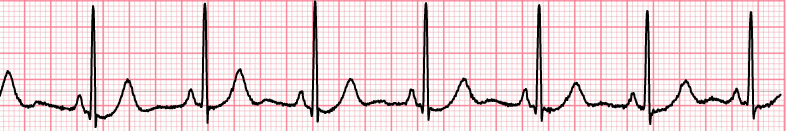
\includegraphics[width=0.8\linewidth, height=0.10\textheight]{ekgexample.png}
        \caption{An example electrokardiogram (EKG).}
\end{figure}
\\
A healthy heartbeat has a fairly regular EKG. As Figure 1 shows, there is a pattern of a quick high voltage followed by small bumps of low voltage. High voltages indicate that the heart is being electrically stimulated, whilst low voltages indicate that the heart is preparing for recovery. 
\begin{figure}[!htb]
    \centering
        \centering
        %\includesvg{integral.svg}
        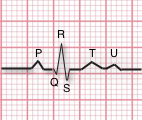
\includegraphics[width=0.4\linewidth, height=0.15\textheight]{ekg.png}
        \caption{An electrokardiogram (EKG) with its waveforms labelled.}
\end{figure}
\\ Figure 2 labels the specific patterns of electrical activity found on an EKG. For example, the sequence $``QRS"$ (also known as the $QRS$-complex) indicates the ventricles of the heart are being stimulated to contract. Sometimes, however, it's possible for the heart to not actually contract during a $QRS$ phase --- a condition known as \emph{electromechanical dissociation}. \\\\
A simplified view treats an EKG as a sequence of the characters `P', `Q', `R', `S', `T', `U', and `-' (where `-' indicates no observable voltage) corresponding to the voltage measurements every millisecond. Then, Figure 2 would be written as the sequence `P-QRS-TU-'. We say that a heartbeat is \emph{regular} if the time between consecutive $R$ voltages is the same; otherwise, the heartbeat is called \emph{irregular}.
\\\\
Given an EKG, can you determine if it corresponds to a heartbeat that is \emph{regular} or \emph{irregular}?
}
\vspace{7mm}\\
\large{\bf{Input}}\vspace{2mm}\\
The input will begin with a line containing a single positive integer, $t$, representing the number of test cases to process. Each test case will consist of a single line containing the characters `P', `Q', `R', `S', `T', `U', and `-'. Every EKG is guaranteed to have at least three $R$ voltages.
\vspace{20mm}\\
\large{\bf{Output}}\vspace{2mm}\\
For each test case print ``Regular" or ``Irregular" on its own line depending on whether the EKG corresponds to a regular or irregular heartbeat.
\vspace{5mm}\\
\bf{Sample Input} \hspace{52mm} \bf{Sample Output}\vspace{1mm}\\
\begin{tabu*} to 475pt {|X[0r]|X[0l]|}
\tabucline-
\vspace{-\baselineskip} %needs to be placed here
\begin{Verbatim}
3
-P-QRSTU-P-QRSTU-P-QRSTU-P-QRSTU
-R---R--R---R-R-------
-R--R--R-----------
\end{Verbatim}
&
\vspace{-\baselineskip} %needs to be placed here
\begin{Verbatim}
Regular
Irregular
Regular
\end{Verbatim}
\\
\tabucline-
\end{tabu*}
\end{document}
